\section{Decision Trees}\label{DecisionTrees} % start a new section and label it for cross-referencing

\subsection{The problem}
Problem: Given a training set D for a target function c, compute the ”best” consistent hypothesis wrt D.


Consider a discrete input space described with $m$ attributes $X = A_1 \times \dots \times A_m$ with A$_{i}$ finite, and a classification problem for f: X $\xrightarrow[]{} C$

The hypothesis space H: set of decision trees.

\subsection{The decision tree}

A decision tree has the following characteristics:
\begin{itemize}
    \item each internal note tests an attribute A$_{i}$ 
    \item each branch denotes a value of an attribute a$_{i,j}$  $\in$ A$_{i}$ 
    \item each leaf node assigns a classification value c $\in$ C
\end{itemize}


\begin{figure}[H]
    \centering
    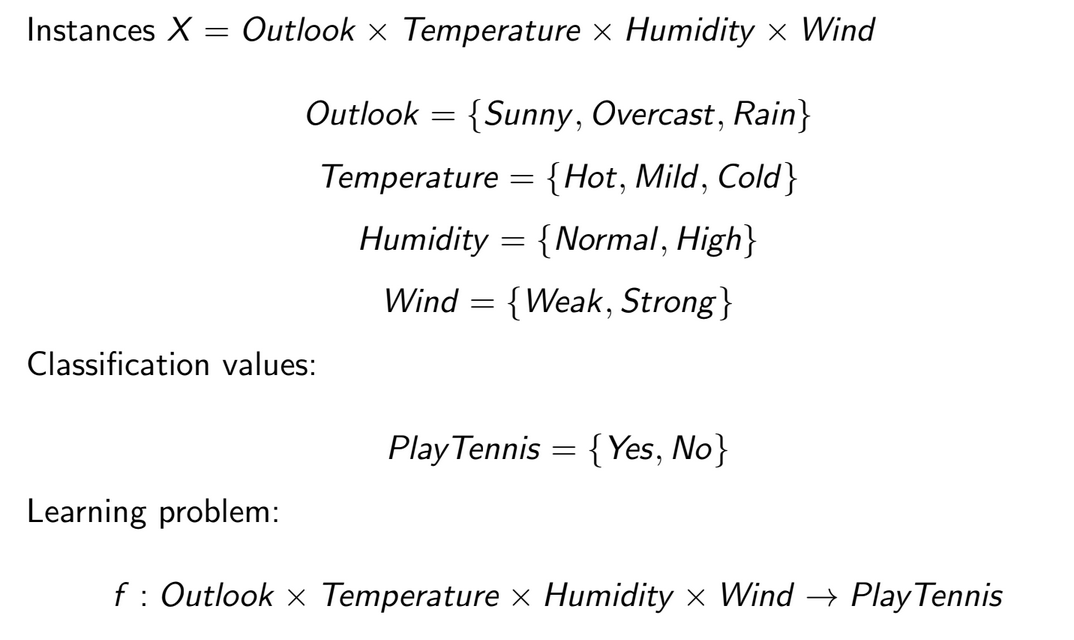
\includegraphics[width=12cm]{images/Decision Trees/Screenshot_20221004_141401.png}
    \caption{}
    \label{fig:image2.1}
\end{figure}

\begin{figure}[H]
    \centering
    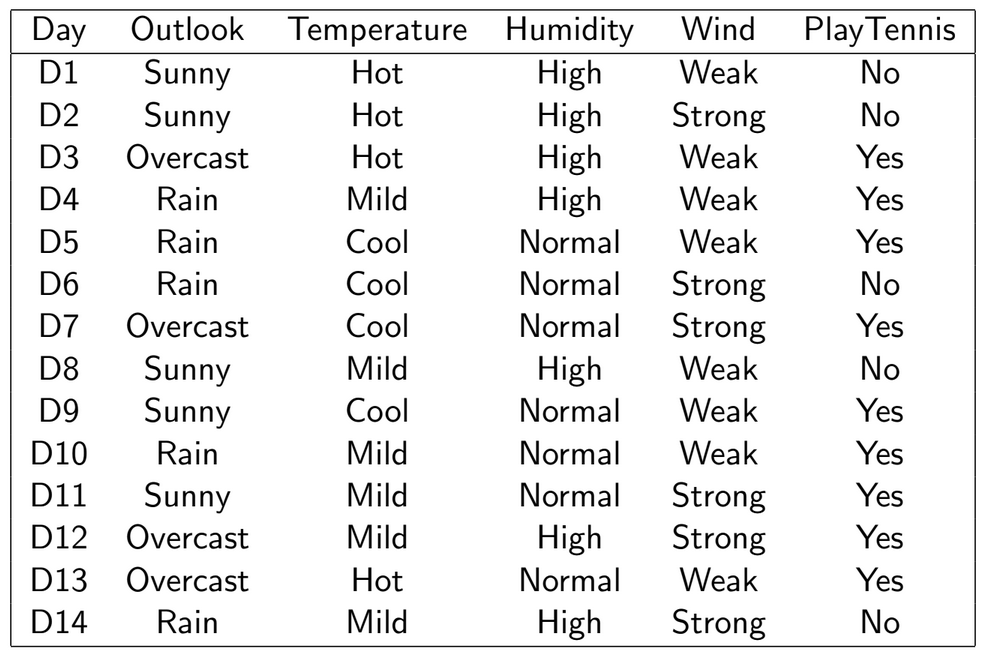
\includegraphics[width=12cm]{images/Decision Trees/Screenshot_20221004_141548.png}
    \caption{}
    \label{fig:image2.2}
\end{figure}


\begin{figure}[H]
    \centering
    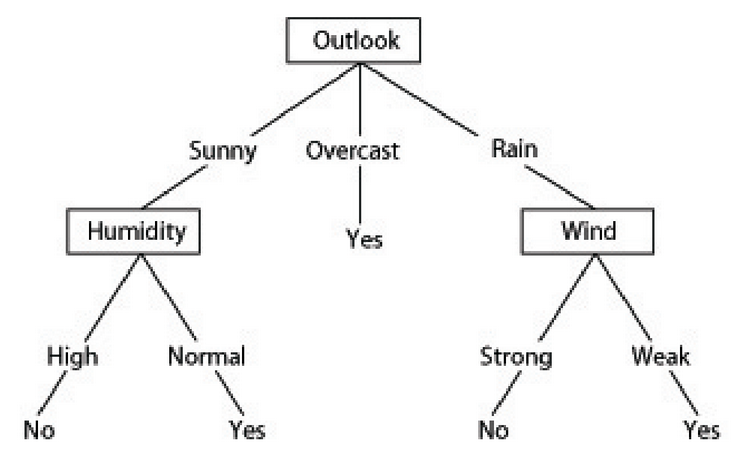
\includegraphics[width=12cm]{images/Decision Trees/Screenshot_20221004_141630.png}
    \caption{}
    \label{fig:image2.3}
\end{figure}

Decision trees represent a disjunction of conjunctions of constraints on the attribute values of instances.

\[(Outlook = Sunny \land Humidity = Normal)\] \[\lor\]
\[(Outlook = Overcast)\] \[\lor\]
\[(Outlook = Rain \land Wind = Weak)\]


\subsection{ID3 Algorithm}
Input: Examples, Target attribute, Attributes \\
Output: Decision Tree
\begin{enumerate}
    \item Create a Root node for the tree
    \item if all Examples are positive, then return the node Root with label +
    \item if all Examples are negative, then return the node Root with label -
    \item if Attributes is empty, then return the node Root with label = most common value of Target attribute in Examples
    \item Otherwise
    \begin{itemize}
        \item A $\xleftarrow[]{}$ the “best” decision attribute for Examples
        \item Assign A as decision attribute for Root
        \item For each value $v_{i}$ of A
         \begin{itemize}
             \item add a new branch from Root corresponding to the test A = $v_{i}$
             \item Examples$_{v_{i}}$ = subset of Examples that have value $v_{i}$ for A
             \item if Examples$_{v_{i}}$ is empty then add a leaf node with label = most common value of Target\_attribute in Examples
             \item else add the tree ID3(Examples$_{v_{i}}$ , Target\_{attribute}, Attributes-{A})
         \end{itemize}
    \end{itemize}
\end{enumerate}

Remember: Output tree depends on attribute order.

We have to measure which attribute gives us the best information

\subsubsection{Information Gain}
Information gain measures how well a given attribute separates the training examples according to their target classification. ID3 selects the attribute that induces highest information gain.

The Information Gain is measured as a reduction in entropy.

\begin{equation}
    Entropy(S) \equiv -p_{\oplus} \log_{2}p_{\oplus} - p_{\ominus} \log_{2}p_{\ominus}
\end{equation}

\begin{figure}[H]
    \centering
    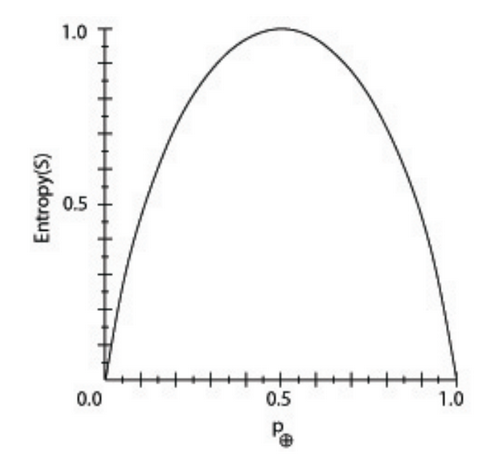
\includegraphics[width=12cm]{images/Decision Trees/Screenshot_20221004_143301.png}
    \caption{}
    \label{fig:image2.4}
\end{figure}

Consider the set S = [9+, 5-] (9 positive examples, 5 negative examples)

\[Entropy(s) = -(9/14)\log_{2}(9/14) -(5/14)\log_{2}(5/14) = 0.940\]


\begin{equation}
    Entropy(S) \equiv \sum_{i=1}^{c}-p_{i}\log_{2}p_{i}
\end{equation}

Now we can calculate the $Gain$, which is by definition the expected reduction in entropy fo S caused by knowing the value of an attribute A.
\begin{equation}
    Gain(S,A) \equiv Entropy(S) - \sum_{v \in Values(A)} \frac{|S_{v}|}{|S|}Entropy(S_v)
\end{equation}
where $Values(A)$ is the set of all possible values of A \\
$S_{v} = {s \in S | A(s) = v}$

\begin{figure}[H]
    \centering
    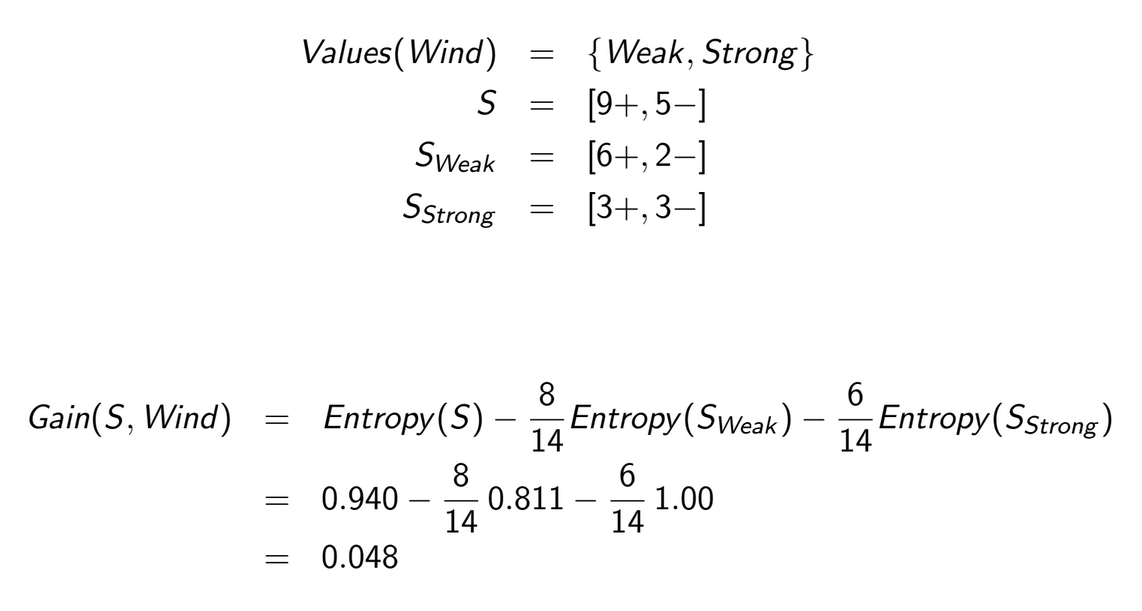
\includegraphics[width=12cm]{images/Decision Trees/Screenshot_20221004_144151.png}
    \caption{}
    \label{fig:image2.5}
\end{figure}

\begin{figure}[H]
    \centering
    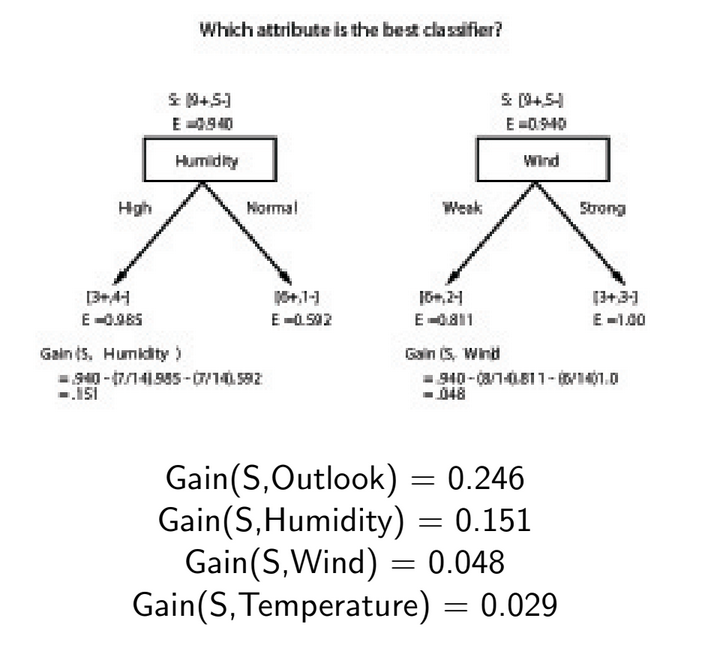
\includegraphics[width=12cm]{images/Decision Trees/Screenshot_20221004_144402.png}
    \caption{}
    \label{fig:image2.6}
\end{figure}

\subsection{Issues in Decision Tree Learning}
Determining how deeply to grow the DT \\
Handling continuous attributes \\
Choosing appropriate attribute selection measures \\
Handling training data with missing attribute values \\
Handling attributes with different costs \\

\vspace{0.5cm}

How can we avoid overfitting?
\begin{itemize}
    \item stop growing when data split not statistically significant
    \item grow full tree, then post-prune
\end{itemize}

To determine the correct tree size:
\begin{itemize}
    \item use a separate set of examples (distinct from the training examples) to evaluate the utility of post-pruning
    \item apply a statistical test to estimate accuracy of a tree on the entire data distribution
    \item using an explicit measure of the complexity for encoding the examples and the decision trees.
\end{itemize}

\subsubsection{Reduced-Error Pruning}

Split data into \emph{training} and \emph{validation} set \\
Do until further pruning is harmful (decreases accuracy):
\begin{itemize}
    \item Evaluate impact on validation set of pruning each possible node (remove all the subtree and assign the most common classification)
    \item Greedily remove the one that most improves validation set accuracy
\end{itemize}

By pruning the tree we are generating smaller and more accurate versions of the tree. Obviously, if the dataset is limited, pruning can led to bad result.

\subsubsection{Continuous variables}
 We can use discrete threshold and set rules based on them. As instance, if we have to measure the temperature, we can st a check "IF temperature > 30C$^{\circ}$"

\subsubsection{Attributes with many values}

We use the $GainRation$ instead

\begin{equation}
    GainRation(S,A) \equiv \frac{Gain(S,A)}{SplitInformation(S,A}
\end{equation}
\begin{equation}
    SplitInformation(S,A) \equiv - \sum_{i = 1}^{c}\frac{|S_{i}|}{|S|} \log_{2}\frac{|S_{i}|}{|S|}
\end{equation}
where $S_{i}$ is subset of S for which A has value $v_{i}$


\subsubsection{Attributes with Cost}

What if Attributes have costs related to them?

we can replace the gain with:
\begin{itemize}
    \item Tan and Schlimmer (1990)
    \begin{equation}
        \frac{Gain^{2}(S,A)}{Cost(A)}
    \end{equation}
    \item Nunez (1988) (w $\in$ [0, 1] determines importance of cost)
    \begin{equation}
        \frac{2^{Gain(S,A)} - 1}{(Cost(A) + 1)^{w}}
    \end{equation}
\end{itemize}

\subsubsection{Unknown Attribute values}

We can use training example anyway, sort through tree
\begin{itemize}
    \item If node n tests A, assign most common value of A among other examples sorted to node n
    \item assign most common value of A among other examples with same target value
    \item assign probability $p_{i}$ to each possible value $v_{i}$ of A
    \begin{itemize}
        \item assign fraction $p_{i}$ of example to each descendant in tree
    \end{itemize}
\end{itemize}

Classify new examples in same fashion

\subsection{Other algorithms based on Decision Trees}
Random Forests: this algorithm generates a collection of decision trees with some random criteria and integrates their values into a final result.

The Random criteria can be: 1) random subsets of data (bagging), 2) random subset of attributes (feature selection) etc.

The Integration of results is made by looking at the majority vote

Random forests are less sensitive to overfitting

